\documentclass[10pt,a4paper]{article}
\usepackage{fullpage}
\usepackage[utf8]{inputenc}
\usepackage[T1]{fontenc}
\usepackage{amsmath}
\usepackage{amssymb}
\usepackage{graphicx}
\usepackage[spanish]{babel}
\usepackage{url}
\usepackage{hyperref}
\usepackage{listings}
\usepackage{textcomp}
\usepackage{accsupp}
\usepackage{attachfile}
\usepackage{verbatim}
\usepackage[misc]{ifsym}
\usepackage{placeins}

% color def
\usepackage{color}
\definecolor{darkred}{rgb}{0.6,0.0,0.0}
\definecolor{darkgreen}{rgb}{0,0.50,0}
\definecolor{lightblue}{rgb}{0.0,0.42,0.91}
\definecolor{orange}{rgb}{0.99,0.48,0.13}
\definecolor{grass}{rgb}{0.18,0.80,0.18}
\definecolor{pink}{rgb}{0.97,0.15,0.45}

% listings
\usepackage{listings}

% General Setting of listings
\lstset{
	language=Python,
	tabsize=4,
	aboveskip=1em,
	breaklines=true,
	abovecaptionskip=0pt,
	captionpos=b,
	escapeinside={\%*}{*)},
	frame=single,
	numbers=left,
	numbersep=8pt,
	numberstyle=\tiny,
	morekeywords=[1]{,as,assert,nonlocal,with,yield,self,True,False,None,} % Python builtin
	morekeywords=[2]{,__init__,__add__,__mul__,__div__,__sub__,__call__,__getitem__,__setitem__,__eq__,__ne__,__nonzero__,__rmul__,__radd__,__repr__,__str__,__get__,__truediv__,__pow__,__name__,__future__,__all__,}, % magic methods
	morekeywords=[3]{,object,type,isinstance,copy,deepcopy,zip,enumerate,reversed,list,set,len,dict,tuple,range,xrange,append,execfile,real,imag,reduce,str,repr,}, % common functions
	morekeywords=[4]{,Exception,NameError,IndexError,SyntaxError,TypeError,ValueError,OverflowError,ZeroDivisionError,}, % errors
	morekeywords=[5]{,ode,fsolve,sqrt,exp,sin,cos,arctan,arctan2,arccos,pi, array,norm,solve,dot,arange,isscalar,max,sum,flatten,shape,reshape,find,any,all,abs,plot,linspace,legend,quad,polyval,polyfit,hstack,concatenate,vstack,column_stack,empty,zeros,ones,rand,vander,grid,pcolor,eig,eigs,eigvals,svd,qr,tan,det,logspace,roll,min,mean,cumsum,cumprod,diff,vectorize,lstsq,cla,eye,xlabel,ylabel,squeeze,}, % numpy / math
	deletekeywords=[2]{next,set,file},
	deletekeywords=[3]{next,set,file},
	basicstyle=\ttfamily,
	backgroundcolor=\color{white},
	commentstyle=\color{darkgreen}\slshape,
	keywordstyle=\color{blue}\bfseries\itshape,
	keywordstyle=[2]\color{blue}\bfseries,
	keywordstyle=[3]\color{grass},
	keywordstyle=[4]\color{red},
	keywordstyle=[5]\color{orange},
	stringstyle=\color{darkred},
	emphstyle=\color{pink}\underbar,
	morestring=[d]{"},
	showstringspaces=false,
	upquote=true,
}



\makeatletter
\lst@RequireAspects{writefile}

% Use \attachfile command to add listing content as paperclip.
\lstnewenvironment{attachedlisting}[1][]{%
	\lst@BeginAlsoWriteFile{#1.txt}%
}
{%
	\lst@EndWriteFile
	\marginpar{\attachfile[appearance=false,icon=Paperclip,mimetype=text/tex]{#1.txt}}
}

% Use accsupp package to add listing content as copyable text.
\lstnewenvironment{copyablelisting}{%
	\lst@BeginAlsoWriteFile{\jobname.txt}%
}
{%
	\lst@EndWriteFile
	\let\verbatim@processline\add@lstline
	\global\let\lstfile\empty
	\verbatiminput{\jobname.txt}%
	\marginpar{(\BeginAccSupp{method=escape,ActualText={\lstfile}}\PaperPortrait\EndAccSupp{})}
}
\def\add@lstline
{\xdef\lstfile{\unexpanded\expandafter{\lstfile}\the\verbatim@line\string^^J}}
\makeatother


\title{{\huge El Juego del Ahorcado}}
\date{}

\begin{document}
\maketitle

\section*{Descripción}
\href{https://es.wikipedia.org/wiki/Ahorcado\_(juego)}{El Ahorcado\footnote{\href{https://es.wikipedia.org/wiki/Ahorcado\_(juego)}{https://es.wikipedia.org/wiki/Ahorcado\_(juego)}}} es un juego rápido y fácil para al menos dos personas que no requiere más que papel, un lápiz y la capacidad de deletrear. Un jugador, el ``anfitrión'', inventa una palabra secreta, mientras que el otro jugador intenta adivinar la palabra preguntando qué letras contiene. Sin embargo, cada intento incorrecto los acerca un paso más a perder. El Ahorcado también se puede personalizar para hacer el juego más fácil, más difícil o educativo, y hay aplicaciones y sitios web para jugar en línea si lo deseas.

\section{El Programa (6 puntos)}
A grandes rasgos, y como ya habrás adivinado, tienes que implementar el juego del ahorcado con Python. Básicamente, consistirá en adivinar una palabra propuesta por tu programa.

Sin embargo, el programa tendrá un menú principal con tres opciones diferentes:
\begin{itemize}
\item Modificar Palabras
\item Jugar
\item Salir
\end{itemize}

\begin{figure}[h!]
\centering
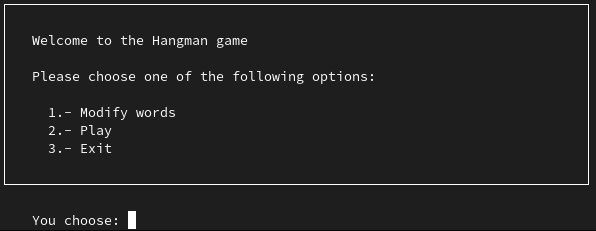
\includegraphics[width=0.9\linewidth]{img/main_menu}
\caption{El menú principal del programa, mostrando las tres opciones.}
\label{fig:main_menu}
\end{figure}

\newpage
\subsection{Modificar Palabras (3 puntos)}
El usuario tiene la oportunidad de gestionar las colecciones de palabras. De esta manera, las palabras se clasifican en categorías que se almacenan en un fichero JSON. Más información sobre el formato JSON se puede encontrar en la Sección~\ref{sec:JSON}. El programa permite al usuario añadir, eliminar y modificar categorías o palabras. Una vez seleccionada esta opción, el programa mostrará el siguiente menú:

\begin{itemize}
\item Añadir categoría
\item Modificar categoría
\item Eliminar categoría
\item Volver al menú principal
\end{itemize}

\begin{figure}[h!]
\centering
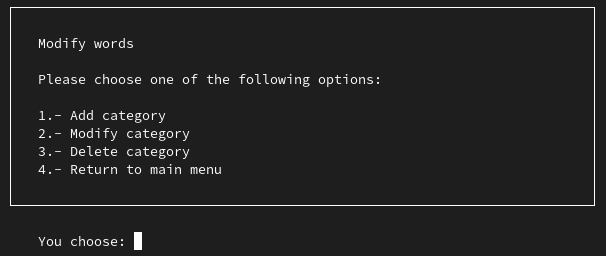
\includegraphics[width=0.8\linewidth]{img/modify_words}
\caption{El menú para modificar las palabras que se usan para jugar.}
\label{fig:modify_words}
\end{figure}

\subsubsection{Agregar Categoría}
Se pedirá al usuario que cree una nueva categoría vacía. Ten cuidado, si la categoría ya existe debes advertir al usuario que el nombre de la categoría no es válido y pedirle un nuevo nombre.

\begin{figure}[h!]
\centering
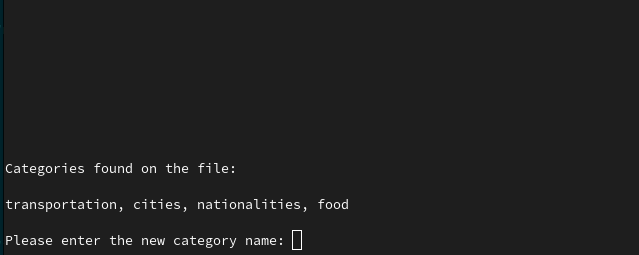
\includegraphics[width=0.8\linewidth]{img/add_category}
\caption{Al añadir una nueva categoría, el programa mostrará al usuario las categorías que están en el fichero y le permitirá introducir una nueva categoría.}
\label{fig:add_category}
\end{figure}

\begin{figure}[h!]
\centering
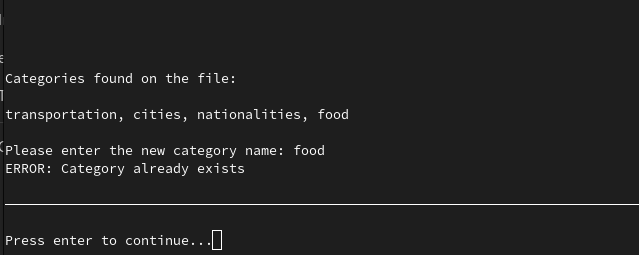
\includegraphics[width=0.8\linewidth]{img/add_category_error}
\caption{Si una categoría ya existe, el programa mostrará un error al usuario.}
\label{fig:add_category_error}
\end{figure}

\newpage
\subsubsection{Modificar Categoría}

El usuario podrá modificar el nombre de la categoría (nuevamente; cuidado con los nombres ya establecidos) o cambiar las palabras de la categoría añadiendo o eliminando una palabra. El nuevo submenú tendrá la siguiente estructura:

\begin{itemize}
\item Cambiar el nombre de la categoría
\item Añadir una nueva palabra
\item Eliminar una palabra
\item Volver al menú anterior
\end{itemize}

El proceso de añadir y, respectivamente, eliminar una palabra de la categoría debe tener en cuenta si la palabra ya estaba almacenada previamente en la categoría dada. La aplicación debe avisar al usuario en consecuencia. Después de cada modificación, el programa debe mostrar al usuario el submenú Modificar Categoría.

\begin{figure}[h!]
\centering
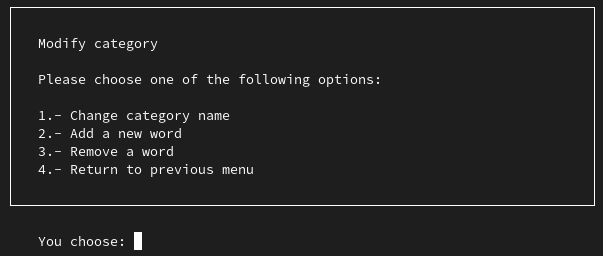
\includegraphics[width=0.9\linewidth]{img/modify_category}
\caption{El menú que muestra las opciones para modificar una categoría.}
\label{fig:modify_category}
\end{figure}

\begin{figure}[h!t]
\centering
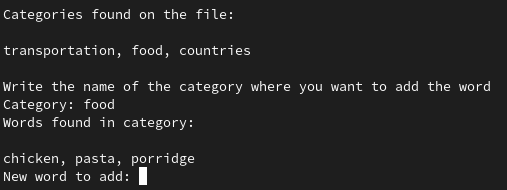
\includegraphics[width=0.9\linewidth]{img/add_word}
\caption{Cada vez que el usuario añada una nueva palabra, primero tendrá que elegir la categoría a la que pertenecerá y luego introducir la palabra.}
\label{fig:add_word}
\end{figure}

\newpage
\subsubsection{Eliminar Categoría}

El programa gestionará la eliminación de categorías. Si la categoría no existe, advertirá al usuario. Además, si la categoría no está vacía, advertirá al usuario que debe eliminar todas las palabras dentro de la categoría primero.

\begin{figure}[h!t]
\centering
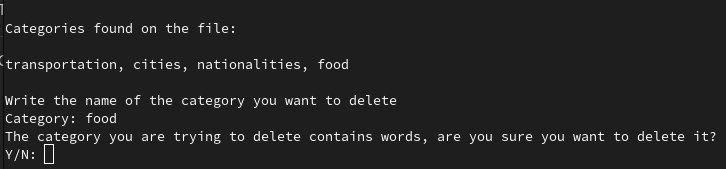
\includegraphics[width=0.9\linewidth]{img/delete_category}
\caption{Para eliminar una categoría, el programa mostrará las categorías disponibles y pedirá al usuario que elija una. Si la categoría que el usuario quiere eliminar contiene alguna palabra, mostrará una advertencia y pedirá al usuario que confirme.}
\label{fig:delete_category}
\end{figure}

\FloatBarrier
\subsection{Jugar (3 puntos)}

Cuando el usuario elige jugar, el programa debe preguntar si el usuario quiere adivinar una palabra al azar o de una categoría dada (nuevamente, el programa advertirá sobre categorías inexistentes). En el primer caso, todas las palabras pueden ser parte de la palabra a adivinar, mientras que en el segundo caso solo aquellas palabras que pertenecen a la categoría mencionada lo serán.

En cada turno, el usuario tendrá que adivinar una letra o la palabra completa. El programa mostrará al usuario las letras que ya ha adivinado y mostrará una advertencia si el usuario usa la misma letra más de una vez. Tendrás que decidir si esto constituirá una vida perdida.

Cuando el usuario adivine la palabra (o no), el programa le dará la oportunidad de jugar de nuevo o volver al menú principal.


\begin{figure}[h!t]
\centering
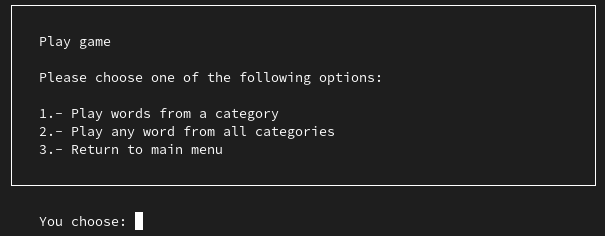
\includegraphics[width=0.9\linewidth]{img/play_game}
\caption{Si el usuario elige jugar, el programa preguntará qué palabras usar.}
\label{fig:play_game}
\end{figure}


\begin{figure}[h!t]
\centering
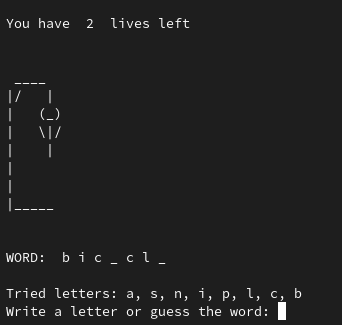
\includegraphics[width=0.7\linewidth]{img/game_advanced}
\caption{Un estado avanzado del juego que muestra las letras que el usuario ya ha adivinado, el estado de la palabra y las vidas que quedan.}
\label{fig:game_advanced}
\end{figure}


\FloatBarrier
\subsection{Salir}

La tercera opción en el menú principal permitirá simplemente que el programa termine normalmente.

\newpage

\section{Manual del Usuario (1 punto)}
Escribe un manual del usuario que describa el juego. En tu manual, explica claramente cómo configurar y ejecutar el juego, comenzando con cualquier instalación necesaria y configuraciones del entorno. Describe la estructura del código, incluyendo una visión general de las funciones principales y cómo interactúan para gestionar la lógica del juego, la interacción del usuario y las condiciones de victoria/derrota. Asegúrate de incluir ejemplos de escenarios típicos de juego, consejos para la resolución de problemas y cualquier modificación que pueda mejorar la experiencia del usuario. Este manual debe estar escrito de manera que tanto los principiantes como los programadores experimentados puedan entender y seguirlo, asegurando que cualquiera que tenga acceso al juego pueda ejecutarlo y apreciar la lógica detrás de su diseño.

Como sugerencia, el manual podría tener secciones para los siguientes elementos:

\begin{enumerate}
\item Explica brevemente el juego del ahorcado, su origen y cómo jugar.
\item Describe cómo lanzar tu programa, incluyendo cualquier módulo necesario que deba ser instalado.
    \begin{itemize}
    \item Si tu programa necesita el fichero de palabras JSON, menciónalo aquí.
    \end{itemize}
\item Explica cómo funciona el juego, los menús que se muestran y cómo interactuar con ellos.
    \begin{itemize}
    \item Recuerda que el programa tiene dos menús principales, uno para modificar el fichero de palabras y otro para jugar.
    \end{itemize}
\item Describe una sesión de juego y las opciones que tiene el usuario.
\end{enumerate}

\section{Algunas Características Adicionales a Considerar (3 puntos)}

Prestaremos especial atención a las siguientes características:

\begin{itemize}
\item Sigues el paradigma de programación estructurada (usando funciones)
\item Asegurate de que el programa tiene comentarios
\item Extiende el programa base con algunas mejoras. Aquí hay algunas sugerencias:
    \begin{itemize}
    \item Verifica si el fichero de palabras existe al principio, y si no, crea uno
    \item Siempre que el usuario tenga que introducir una categoría o palabra, haz que la elija de una lista enumerada, como con los menús
    \item Añade varios niveles de dificultad cambiando la cantidad de vidas iniciales
    \item Añade niveles de dificultad para las palabras
    \item Lleva un registro del número de aciertos por parte de los usuarios o dales puntos según la cantidad de vidas restantes
        \begin{itemize}
        \item Almacena esos puntos con su nombre de usuario en un fichero para que sean persistentes
        \end{itemize}
    \end{itemize}
\end{itemize}

\newpage

\section{Formato JSON}
\label{sec:JSON}

JSON (JavaScript Object Notation) es un formato de datos ligero y basado en texto que es fácil de leer y escribir tanto para humanos como para máquinas. Se usa comúnmente para el intercambio de datos entre aplicaciones. JSON representa datos en pares clave-valor, similar a los diccionarios de Python, y admite estructuras anidadas como arrays (listas) y objetos (diccionarios). El Listing~\ref{lst:json} contiene un ejemplo de cadena formateada como JSON.

Los tipos de datos disponibles en una cadena JSON son los siguientes:

\begin{description}
\item[Objeto:] Los pares $<clave, valor>$, similar a un \lstinline|dict|
\item[Número:] Un número, similar a un \lstinline|float|
\item[Cadena:] Una secuencia de caracteres delimitada por comillas dobles
\item[Booleano:] Un valor \lstinline|true| o \lstinline|false|
\item[Array:] Una lista ordenada de elementos, similar a \lstinline|list|
\item[nulo:] Un valor vacío, similar a \lstinline|None|
\end{description}

\begin{lstlisting}[caption={Ejemplo de cadena formateada como JSON.}, label=lst:json]
{
  "first_name": "John",
  "last_name": "Smith",
  "is_alive": true,
  "age": 27,
  "address": {
    "street_address": "21 2nd Street",
    "city": "New York",
    "state": "NY",
    "postal_code": "10021-3100"
  },
  "phone_numbers": [
    {
      "type": "home",
      "number": "212 555-1234"
    },
    {
      "type": "office",
      "number": "646 555-4567"
    }
  ]
}
\end{lstlisting}

En Python, puedes trabajar con ficheros JSON con el módulo \texttt{json}. No es necesario instalar nada, solo tienes que importarlo. Aquí tienes una breve descripción de cómo usar JSON en Python:

\subsection{Lectura de Ficheros JSON}
Abre el fichero JSON y usa \lstinline|json.load()| para convertir su contenido en un diccionario de Python.

\begin{lstlisting}
import json

with open('words.json', 'r') as file:
    data = json.load(file)
print(data)
\end{lstlisting}

\subsection{Escritura de Ficheros JSON}
Usa \lstinline|json.dump()| para convertir un diccionario de Python a una cadena formateada como JSON y escribirla en un fichero.

\begin{lstlisting}
import json

data = {'name': 'Alice', 'age': 30, 'city': 'Wonderland'}
with open('data.json', 'w') as file:
    json.dump(data, file, indent=4)
\end{lstlisting}

\subsection{Análisis de Cadenas JSON}
Si tienes una cadena JSON, puedes convertirla en un objeto de Python usando \lstinline|json.loads()|.

\begin{lstlisting}
import json

json_str = '{"name": "Alice", "age": 30, "city": "Wonderland"}'
data = json.loads(json_str)
print(data)
\end{lstlisting}

\subsection{Conversión de Objetos de Python a Cadenas JSON}
Usa \lstinline|json.dumps()| para convertir un objeto de Python en una cadena formateada como JSON.

\begin{lstlisting}
import json

data = {'name': 'Alice', 'age': 30, 'city': Wonderland'}
json_str = json.dumps(data, indent=4)
print(json_str)
\end{lstlisting}

\subsection{Páginas web para Jugar con JSON}
Hay algunas páginas web que te ayudarán a visualizar mejor la estructura JSON.

\begin{itemize}
\setlength\itemsep{0.4cm}
\item \href{http://www.json.org/json-en.html}{\color{blue}\underline{http://www.json.org/json-en.html}}
\item \href{https://codebeautify.org/jsonviewer}{\color{blue}\underline{https://codebeautify.org/jsonviewer}}
\item \href{http://jsonviewer.stack.hu/}{\color{blue}\underline{http://jsonviewer.stack.hu/}}
\item \href{https://jsongenerate.com/visualizer}{\color{blue}\underline{https://jsongenerate.com/visualizer}}
\end{itemize}

\end{document}